\documentclass[border=4pt]{standalone}
\usepackage[T1]{fontenc}
\usepackage{helvet}
\renewcommand{\familydefault}{\sfdefault}
\usepackage{tikz}
\usetikzlibrary{positioning,arrows.meta,calc,fit,backgrounds}
\definecolor{ink}{HTML}{2C3138}
\definecolor{ink2}{HTML}{52514E}
\definecolor{pblue}{HTML}{EAF3FC}
\definecolor{pblueline}{HTML}{7CB6F1}
\definecolor{prose}{HTML}{FBEDEB}
\definecolor{proseline}{HTML}{D99A93}
\definecolor{pgreen}{HTML}{EEF6E9}
\definecolor{pgreenline}{HTML}{94C07C}
\definecolor{plav}{HTML}{F1ECFB}
\definecolor{plavline}{HTML}{B59BE6}
\definecolor{papri}{HTML}{FCF1E9}
\definecolor{papriline}{HTML}{E3A072}
\definecolor{pgold}{HTML}{F8F3E4}
\definecolor{pgoldline}{HTML}{CBAE5E}
\definecolor{pband}{HTML}{F3F4F6}
\begin{document}
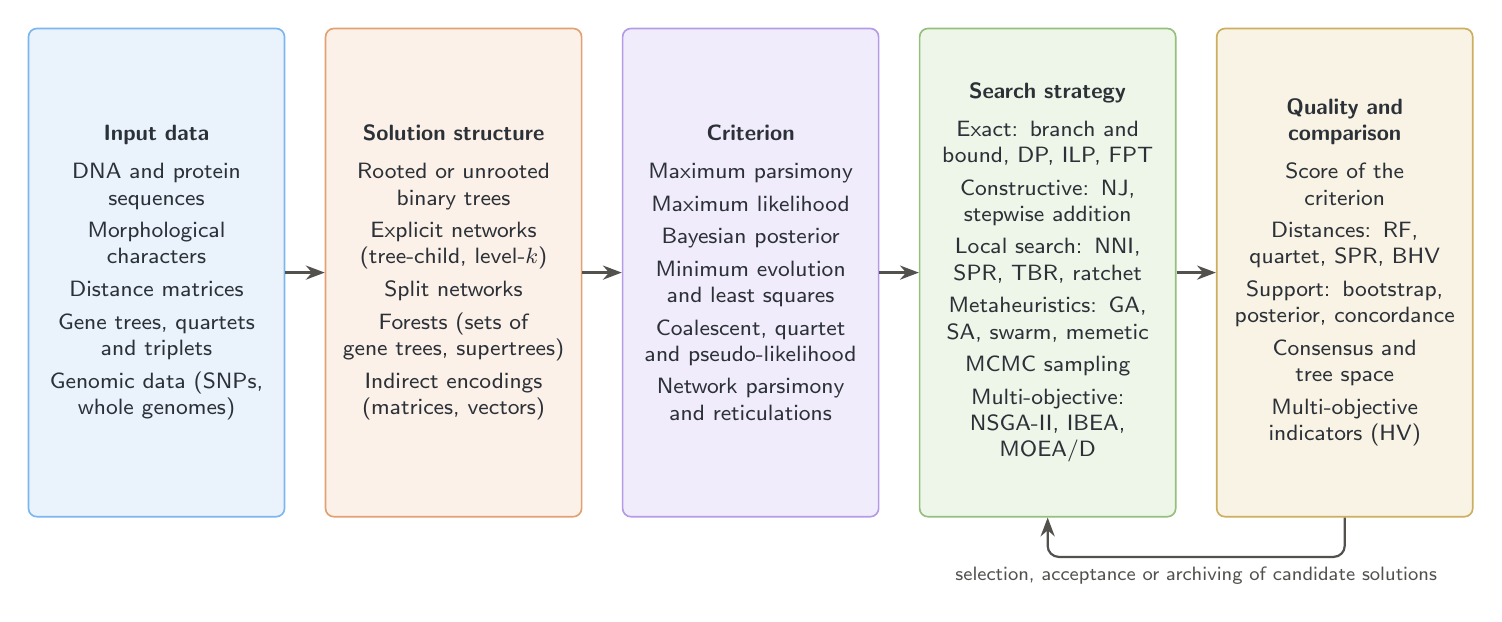
\begin{tikzpicture}[font=\footnotesize, text=ink, node distance=5mm,
  col/.style={rounded corners=3pt, align=center, text width=29mm, minimum height=62mm, inner sep=5pt, line width=0.6pt},
  arr/.style={-{Stealth[length=2.4mm]}, draw=ink2, line width=0.8pt}]
\node[col, draw=pblueline, fill=pblue] (data) {\textbf{Input data}\\[1.5mm] DNA and protein\\sequences\\[0.8mm] Morphological\\characters\\[0.8mm] Distance matrices\\[0.8mm] Gene trees, quartets\\and triplets\\[0.8mm] Genomic data (SNPs,\\whole genomes)};
\node[col, draw=papriline, fill=papri, right=of data] (sol) {\textbf{Solution structure}\\[1.5mm] Rooted or unrooted\\binary trees\\[0.8mm] Explicit networks\\(tree-child, level-$k$)\\[0.8mm] Split networks\\[0.8mm] Forests (sets of\\gene trees, supertrees)\\[0.8mm] Indirect encodings\\(matrices, vectors)};
\node[col, draw=plavline, fill=plav, right=of sol] (crit) {\textbf{Criterion}\\[1.5mm] Maximum parsimony\\[0.8mm] Maximum likelihood\\[0.8mm] Bayesian posterior\\[0.8mm] Minimum evolution\\and least squares\\[0.8mm] Coalescent, quartet\\and pseudo-likelihood\\[0.8mm] Network parsimony\\and reticulations};
\node[col, draw=pgreenline, fill=pgreen, right=of crit] (search) {\textbf{Search strategy}\\[1.5mm] Exact: branch and\\bound, DP, ILP, FPT\\[0.8mm] Constructive: NJ,\\stepwise addition\\[0.8mm] Local search: NNI,\\SPR, TBR, ratchet\\[0.8mm] Metaheuristics: GA,\\SA, swarm, memetic\\[0.8mm] MCMC sampling\\[0.8mm] Multi-objective:\\NSGA-II, IBEA, MOEA/D};
\node[col, draw=pgoldline, fill=pgold, right=of search] (qual) {\textbf{Quality and comparison}\\[1.5mm] Score of the\\criterion\\[0.8mm] Distances: RF,\\quartet, SPR, BHV\\[0.8mm] Support: bootstrap,\\posterior, concordance\\[0.8mm] Consensus and\\tree space\\[0.8mm] Multi-objective\\indicators (HV)};
\draw[arr] (data) -- (sol); \draw[arr] (sol) -- (crit); \draw[arr] (crit) -- (search); \draw[arr] (search) -- (qual);
\draw[arr, rounded corners=4pt] (qual.south) -- ++(0,-5mm) -| node[pos=0.25, below, font=\scriptsize, text=ink2] {selection, acceptance or archiving of candidate solutions} (search.south);
\end{tikzpicture}
\end{document}
